\documentclass[twocolumn]{IEEEtran}
\usepackage{epsfig}
\usepackage{url}
\usepackage{graphicx}
\usepackage{float}
%-----------------------

\begin{document}
\title{CACHEOMS: Practical Exploitation of \textbf{Cache} Side Channel \textbf{O}n \textbf{M}ultiprocessor \textbf{S}ystems}


\author{Aravind Machiry \& Varun Kulkarni Somashekhar
\thanks{Authors are with the
Department of Computer Science,
University of California, Santa Barbara, CA 93106.
E-mail: \texttt{\{machiry,varun\_kulkarni\}@cs.ucsb.edu}}
}

\maketitle

\begin{abstract}
Cache side channel is well known attack on cryptographic implementations\cite{bernstein2005cache}\cite{aciccmez2006trace}\cite{banescu2011cache}. This is primarily based on observation that infrequently used information incurs a large timing penalty, thus revealing some information about the frequency of use of the memory blocks. This attack is straight forward on a single processor system with single level of cache, but current systems (both desktop and mobile) are multiprocessor where each processor has multilevel caches also there are some cache levels which are common to a subset of processors. Moreover, latest ARM processors have TrustZone support\cite{frenzel2010arm} which ensures System-On-Chip (SOC) wide security by avoiding shared cache access. In addition to this, there has been lot of work done both on Hardware and Software side to mitigate cache side channel\cite{180212}\cite{wang2007new}. It is high time we revisit and evaluate cache side channel, its possibility on latest processors and implications\cite{184415}.\\
\end{abstract}

\section {Introduction}
Memory access time is the main bottleneck for achieving maximum processor performance. Memory hierarchies are used to bridge this gap. Memory cache is the main component of the hierarchy. Most of the Processors have memory caches whose access time is several times less than main memory. On latest Intel I7 processor, access to L1 cache takes ~2 cycles, where as it takes ~360-400 cycles to access a byte from main memory. Memory Caches are continuously evolving and lot of research have been done to make these as fast as the corresponding processor. On the other hand, main memory access time is not decreasing accordingly. This makes an access to main memory to be easily distinguishable by measuring access time. The difference in the access time is the main idea based on which most of the cache side channel attacks are discovered. Recent improvements in cache technologies seems to decrease cache access time thus making main memory access extremely easy to detect. 

All known attacks are implemented on previous generation processors like Pentium III (cite from challenges), Pentium 4E (cite from challenges) and Athlon 64 (cite from challenges). Although, recent improvements in caches make cache side attacks more reliable, multi-core processors with multiple levels of cache makes exploiting cache side-channels non trivial. Moreover, recent processors have pre-fetching\cite{tse1998cpu} which thwarts most of the known attacks. In this project, we explore the feasibility cache timing attacks on latest multiprocessor based systems, discuss our findings and results. Specifically, following are our contributions:
\begin{itemize}
\item Investigate, understand and report cache side channel with examples. We aim to make the documentation simple enough to be understood by a computer science graduate without much knowledge of cryptography or computer architecture.
\item Implement cache timing attack on Latest Intel i7-930 processor and report our findings.
\item Investigate and report existing defense strategies to prevent cache side channel.
\end{itemize}


\section {Background}

In this section we give a brief overview of the background needed to understand the attack presented in this work. After summarizing the design of cache architecture, a short explanation about different types of cache attacks are provided.

\subsection {Cache Design and Operation}

A cache is a small memory placed between the CPU and RAM to reduce the big latency added by retrieval of data. Modern processors usually have more than one level of cache to improve the efficiency of memory access. Most modern processes offer 3 levels of cache.with the first level (L1) being the closest to the CPU registers. Generally, L1 and L2 caches are each split into instruction caches and separate data caches. L3 usually stores both instructions and data.The cache size is much smaller than the number of directly addressable bytes in main memory. Hence a mapping strategy needs to be adopted.The cache associativity determines how the main memory blocks map into blocks of the cache. The below figure depicts the differences between direct mapped cache and an associative cache memory

\begin{figure}[H]
  \centering
  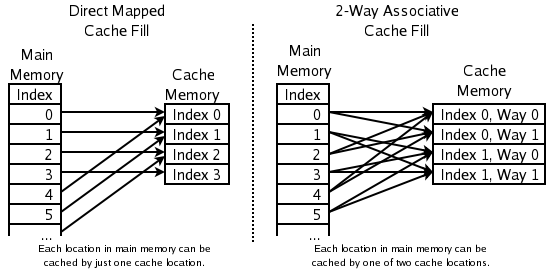
\includegraphics[width=90mm]{cache}
\end{figure}

Each block in the cache is in one of the below four states:

\begin {itemize}
\item \textbf {Invalid:} This block has an incoherent copy of the memory.
\item \textbf{Valid:} This block has a coherent copy of the memory. The data may be possibly shared, but its content is not modified.
\item \textbf{Reserved:} The block is the only copy of the memory, but it is still coherent. No write back is needed if the block is replaced.
\item \textbf {Dirty:} The block is the only copy of the memory and it is incoherent. This copy was written one or more times. This is the only state that generates a write-back when the block is replaced in the cache.

\end{itemize}


\begin{figure}[H]
  \centering
  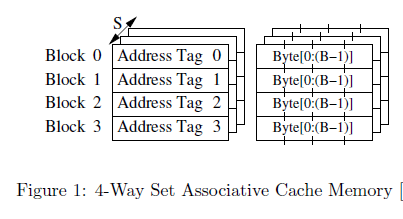
\includegraphics[width=90mm]{2}
\end{figure}

 A cache is divided into blocks  of fixed size (B bytes).  Blocks, are grouped into a number (S) of sets such that each set has an equal number of blocks. The number (W) of blocks in a set denotes the associativity of a cache, and is usually a small power
of 2. The total cache size is: $S\times W\times B$  bytes.


More specifically, if we have a 4-way set associative cache like in Figure 1, then a main memory block can map to any of the 4 blocks of a given set. The set corresponding to a main memory block is determined from its physical address by splitting it into:

\begin {itemize}
\item a \textbf{tag address} taking $\log \frac{N}{S\times B}$  bits from the most significant part of the address;
\item a \textbf{set number} taking $\log {S}$ bits from the middle part of the physical address;
\item a\textbf{ block offset} taking $\log {B}$ bits from the least significant part of the physical address
\end{itemize}


When a memory reference is made by the CPU, the tag address of the main memory block is compared with all the tags in the corresponding set. If the tag is found then this reference qualifies as a cache hit. Meaning that there is no need to retrieve the data from main memory since it is already located in the cache, and the data can be immediately provided to the CPU. Conversely, if the tag is not found in the corresponding set then the memory reference qualifies as a cache miss.The caching mechanism operation is based on the principals of spatial and temporal locality, which help to minimize the number of
cache misses. Temporal locality states that the same data blocks will likely be requested repeatedly during the execution of a process. Spacial locality states that data blocks from nearby addresses are likely to be subsequently accessed. Even though the number of cache misses is reduced by these principles, they are not eliminated.

Obviously, data in the cache can be accessed much faster than data present only in memory.This is also true for multi-level caches where data accessed from the L1 cache will experience lower latencies, than data accessed from subsequent cache levels. These time differences are used to decide whether a specific portion of memory resides in the cache - implying that the corresponding data has been accessed recently. This resulting information leakage stemming from microarchitectural time differences when data is retrieved from cache rather than memory forms the basis of cache side channel attacks.

\subsection { Types of Cache Side Channel Attacks }

Cache misses occur at every cache level and they are categorized as:

\begin {itemize}
\item \textbf{cold start misses}, which occur when data is first referenced;
\item \textbf{capacity misses}, which occur if the size of the LUTs Look Up Table used by the cipher is larger than the size of the cache; this type of cache misses do not occur for most cryptographic cipher implementations.
\item \textbf{conflict misses}, which occur when at least two elements of LUTs that map to the same cache block are used.
\end {itemize}

Based on this idea, cache attacks can be classified into three groups:

\begin {itemize}

\item \textbf{Reset attacks} require that all or most LUTs used by the cryptographic cipher are not to be loaded in the cache before the attack commences. Therefore this type of attacks is mainly based on cold start misses.

\item \textbf{Initialization attacks} require the adversary to be able to set the cache into a known state before the attack commences. Therefore this type of attacks is based both on cold start misses and conflict misses.

\item \textbf{Micro-architecture attacks} require the cache to hold all or most LUTs that will be used by the cipher,before the attack commences. Therefore this type of attacks is partially based only on conflict misses and partially on other timing penalties that
strongly depend on the CPU micro-architecture. 

\end {itemize}

These three types of attacks are not limited to timing channels. Measuring power dissipation levels during the encryption process also offers more information about data access. However, this work would focus only on timing attacks.

\section {Attack Implementation}
In this section, we explain our implementation of an attack based on cache timing on Intel i7-930 processor. First, we describe the cache organization on this processor. Second, we explain our attack goal and strategy. Finally, we describe our implementation.
\subsection {Cache Organization}
Processor Intel i7-930 has 4 physical cores and has Hyper-threading support\cite{intelhype}, which exposes 8 (4 * 2) virtual cores. Cache on the processor has 3 levels, which is shared among these 8 virtual cores. Organization of various cache levels and corresponding properties is as shown in the below Table:
\begin{center}
\scalebox{0.5}{
\begin{tabular}{ |c|c|c|c|c|c|c| } 
 \hline
 Cache Level & Type & Shared Virtual Cores & Size(Bytes) & Sets & Associativity & Line Size(Bytes)\\
 \hline
 L1 & Data & 0,4  & 32K & 64 & 8 & 64 \\
 L1 & Instruction & 0,4 & 32K & 64 & 8 & 64 \\
 L1 & Data & 1,5  & 32K & 64 & 8 & 64 \\
 L1 & Instruction & 1,5 & 32K & 64 & 8 & 64 \\
 L1 & Data & 2,6  & 32K & 64 & 8 & 64 \\
 L1 & Instruction & 2,6 & 32K & 64 & 8 & 64 \\
 L1 & Data & 3,7  & 32K & 64 & 8 & 64 \\
 L1 & Instruction & 3,7 & 32K & 64 & 8 & 64 \\
 \hline
 L2 & Unified & 0,4  & 256K & 512 & 8 & 64 \\
 L2 & Unified & 1,5  & 256K & 512 & 8 & 64 \\
 L2 & Unified & 2,6  & 256K & 512 & 8 & 64 \\
 L2 & Unified & 3,7  & 256K & 512 & 8 & 64 \\
 \hline
 L2 & Unified & All & 8192K & 8192 & 16 & 64 \\
 \hline
\end{tabular}
}
\end{center}
Most of the known methods to find cache information of a system requires additional (usually $\texttt{root}$) privileges. However we wrote a python script($\texttt{get\_cpu\_cache\_info.py}$) which get details of entire cache organization of any system running *nix operating system, moreover $\textit{this script doesn't require \texttt{root} privileges}$. As you can see cache organization is non trivial, you may or may not be able to exploit cache timing side channel depending on virtual cores on which attack and victim process gets executed. Also note that cache sizes are considerably larger then key size of most of the cryptographic algorithms, which makes attacks based on capacity misses practically impossible.
\subsection {Attack Goal and Strategy}
In this subsection, we explain goal of the attack and strategy we used to perform the attack.
\subsubsection {Attack Goal}
The goal of the attack is to predict the cache set of a data item which the victim process is repeatedly accessing. To emulate the possibility of attacker ability to measure memory access time, the victim process outputs access time of the data item.
\subsubsection {Strategy}
Our strategy is to exploit delay due to conflict misses. Specifically, we launch an attack process which tries to fill up one cache set at a time. If the data item of victim process maps to the same cache set then we should see considerable increase in access time, otherwise access time should not be affected. We repeat this for all the sets in the cache and observe the access time of victim process, an increase in access time implies the cache set filled by attack process is same as the cache set of the data item which the victim process is trying to access.
\subsection {Implementation}
We measured the access time of data item as seen by a process(p1) when another process(p2) is trying to access data that belongs to both same and different cache set. We see following differences:
\begin{center}
\scalebox{0.4}{
\begin{tabular}{p{5cm}p{5cm}p{5cm}p{5cm}}
\hline
Description & P1 Data item set & P2 Data item set & P1 Access Time\\
\hline
P2 Doesn't access any data & x & N/A & {\bf 6 ns}\\
\hline
P2 Access data belongs to different cache set as P1 data & x & y (y$\neq$x) & {\bf 8-9ns} \\
\hline
P2 Access data that belongs to same cache set as P1 data & x & x & {\bf 10-11 ns}\\
\hline
\end{tabular}
}
\end{center}
\begin{figure}[H]
  \centering
  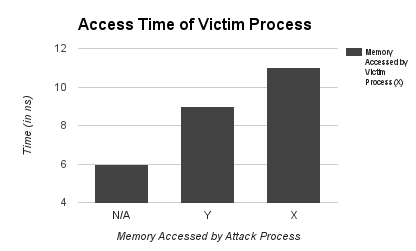
\includegraphics[width=90mm]{chart}
\end{figure}
The chart above shows graphical representation of access time difference. We expected access time to be same for first and second bar in the chart, as they should not affect access time for victim process, but the reason they are different is because of simultaneous access to cache. L1-Cache allows a single access per clock, thus when multiple process tries to access same cache module, they will be serialized and thus the delay. But the delay is quite noticeable in Row 3 when both process tries to access same cache set. This delay is due to L1-Cache miss penalty. Our idea is to run a process which tries to fill up an entire cache set and measure the delay experienced by victim process. If the set is same then the delay should be atleast 10 ns. We have implemented this attack in C and wrote a single wrapper python script $\texttt{l1\_timing\_attack.py}$ which drives the attack and provides the result.
\section {Defence}
There have been many defences developed in both Hardware and Software to protect against all Cache side channel attacks. This section briefly describes them and suggest the reader to refer the cited work for more details. Cache interference is the general term used to describe all side channels because of shared cache.
\subsection {Hardware Defences}
In this section, we briefly explain existing Hardware defences\cite{wang2007new}.
\begin{itemize}
\item \textbf {Partition Locked Cache} essentially achieves the effect of cache partitioning, but much more flexibly with less performance degradation. In partition locked cache, the cache lines of interest are locked in cache, creating a flexible private partition; these cache lines can not be evicted by other cache accesses not belonging to this private partition. This prevents both internal and external cache interferences.

\item \textbf {Random Permutation Cache} allows cache sharing by randomizing the resulting interference, so that no useful information about which cache line was evicted can be inferred. An attacker can observe another process’s cache access only if that process changes the attacker’s cache usage, i.e., evicts the attacker’s cache lines. If the process evicts its own cache lines, the attacker has no way to know that.  In random permutation cache, each time cache interference occurs, the interference is randomized in a way that carries no useful information. 

\item \textbf{ARM TrustZone}\cite{frenzel2010arm} is a system-wide protection mechanism introduced by ARM. It provides two virtual processors backed by hardware based access control. This lets the application core switch between two states, referred to as worlds (to reduce confusion with other names for capability domains), in order to prevent information from leaking from the more trusted world to the less trusted world. This world switch is generally orthogonal to all other capabilities of the processor, thus each world can operate independently of the other while using the same core. Memory and peripherals are then made aware of the operating world of the core and may use this to provide access control to secrets and code on the device. \\
Cache is not shared between 2-worlds, thus all the sensitive process can run in secure world thus thwarting all interference attacks.

\end{itemize}
\subsection {Software Defences}
In this section, we briefly explain most commonly used software defences:
\begin{itemize}
\item \textbf{Random Delay} Since most of the attacks rely on timing difference to be successful, sensitive process can introduce random delay to hinder these at the cost of computation delay.
\item \textbf{Dynamic Software Diversity}\cite{crane2015thwarting} In this technique, we create a large number of unique program execution paths by automatically generating diversified replicas for parts of an input program. Replicas derived from the same original program  fragment have different implementations, but perform semantically equivalent computations. At runtime we then randomly and frequently switch between these replicas.
\end{itemize}

\section {Conclusion and Future Work}

The attack strategies as illustrated in the preceding sections are very simple to implement even in modern processors. However there are several constraints such as  the attacker and victim process should be scheduled on the same core so that shared L1 cache can be exploited for cache interferences. Even in cases where the attacker and victim processes are on different cores, a similar kind of attack can be constructed  based on cache interferences in the shared L3 cache. Such attacks have been discussed in detail in \cite{sc2015lastlevel}. Our work concentrates primarily on shared L1 caches. These attacks can be extended to break cipher implementations based on LUTs namely AES and DES. Due to heirarchical memory model, subsequent access to LUT's are performed in variable amounts of time resulting in leakage of side channel information. Once the attacker gets an approximate idea the size of look up table in the cache set based on cache evictions, he can then resort to brute force to determine the key for the corresponding cipher implementation.

The same methodology can be employed in the cloud wherein the virtual machines co-resident on the same core display similar behavior and thus leak side channel information. Several such attempts have been successful and have been discussed in  \cite{sc2015lastlevel}.  Similar strategies can be constructed to perform a shared cache attack that work across cores and has been discussed recently in \cite{ir2015aes}.



\bibliographystyle{IEEEbib}
\bibliography{my}

\end{document}

